\documentclass[11pt]{article}
% 用ctex显示中文并用fandol主题
\usepackage[fontset=fandol]{ctex}
\setmainfont{CMU Serif} % 能显示大量外文字体
\xeCJKsetup{CJKmath=true} % 数学模式中可以输入中文

% AMS全家桶,\DeclareMathOperator依赖之
\usepackage{amsmath,amssymb,amsthm,amsfonts,amscd}
\usepackage{pgfplots,tikz,tikz-cd} % 用来画交换图
\usepackage{bm,mathrsfs} % 粗体字母(含希腊字母)和\mathscr字体
\everymath{\displaystyle} % 全体公式为行间形式

% 纸张上下左右页边距
\usepackage[a4paper,left=1cm,right=1cm,top=1.5cm,bottom=1.5cm]{geometry}
% 生成书签和目录上的超链接
\usepackage[colorlinks=true,linkcolor=blue,filecolor=blue,urlcolor=blue,citecolor=cyan]{hyperref}
% 各种列表环境的行距
\usepackage{enumitem}
\setenumerate[1]{itemsep=0pt,partopsep=0pt,parsep=\parskip,topsep=0pt}
\setenumerate[2]{itemsep=0pt,partopsep=0pt,parsep=\parskip,topsep=0pt}
\setenumerate[3]{itemsep=0pt,partopsep=0pt,parsep=\parskip,topsep=0pt}
\setitemize[1]{itemsep=0pt,partopsep=0pt,parsep=\parskip,topsep=5pt}
\setdescription{itemsep=0pt,partopsep=0pt,parsep=\parskip,topsep=5pt}
\setlength\belowdisplayskip{2pt}
\setlength\abovedisplayskip{2pt}

% 左右配对符号
\newcommand{\br}[1]{\!\left(#1\right)} % 括号
\newcommand{\cbr}[1]{\left\{#1\right\}} % 大括号
\newcommand{\abr}[1]{\left<#1\right>} % 尖括号(内积)
\newcommand{\bbr}[1]{\left[#1\right]} % 中括号
\newcommand{\abbr}[1]{\left(#1\right]} % 左开右闭区间
\newcommand{\babr}[1]{\left[#1\right)} % 左闭右开区间
\newcommand{\abs}[1]{\left|#1\right|} % 绝对值
\newcommand{\norm}[1]{\left\|#1\right\|} % 范数
\newcommand{\floor}[1]{\left\lfloor#1\right\rfloor} % 下取整
\newcommand{\ceil}[1]{\left\lceil#1\right\rceil} % 上取整
% 常用数集简写
\newcommand{\R}{\mathbb{R}} % 实数域
\newcommand{\N}{\mathbb{N}} % 自然数集
\newcommand{\Z}{\mathbb{Z}} % 整数集
\newcommand{\C}{\mathbb{C}} % 复数域
\newcommand{\F}{\mathbb{F}} % 一般数域
\newcommand{\kfield}{\Bbbk} % 域
\newcommand{\K}{\mathbb{K}} % 域
\newcommand{\Q}{\mathbb{Q}} % 有理数域
\newcommand{\Pprime}{\mathbb{P}} % 全体素数,或概率
% 范畴记号
\newcommand{\Ccat}{\mathsf{C}}
\newcommand{\Grp}{\mathsf{Grp}} % 群范畴
\newcommand{\Ab}{\mathsf{Ab}} % 交换群范畴
\newcommand{\Ring}{\mathsf{Ring}} % (含幺)环范畴
\newcommand{\Set}{\mathsf{Set}} % 集合范畴
\newcommand{\Mod}{\mathsf{Mod}} % 模范畴
\newcommand{\Vect}{\mathsf{Vect}} % 向量空间范畴
\newcommand{\Alg}{\mathsf{Alg}} % 代数范畴
\newcommand{\Comm}{\mathsf{Comm}} % 交换
% 代数集合
\DeclareMathOperator{\Hom}{Hom} % 同态
\DeclareMathOperator{\End}{End} % 自同态
\DeclareMathOperator{\Iso}{Iso} % 同构
\DeclareMathOperator{\Aut}{Aut} % 自同构
\DeclareMathOperator{\Inn}{Inn} % 内自同构
% \DeclareMathOperator{\inv}{Inv}
\DeclareMathOperator{\GL}{GL} % 一般线性群
\DeclareMathOperator{\SL}{SL} % 特殊线性群
\DeclareMathOperator{\GF}{GF} % Galois域
% 正体符号
\renewcommand{\i}{\mathrm{i}} % 本产生无点i
\newcommand{\id}{\mathrm{id}} % 恒等映射
\newcommand{\e}{\mathrm{e}} % 自然常数e
\renewcommand{\d}{\mathrm{d}} % 微分符号,本产生重音符号
\newcommand{\D}{\partial} % 偏导符号
\newcommand{\diff}[2]{\frac{\d #1}{\d #2}}
\newcommand{\Diff}[2]{\frac{\D #1}{\D #2}}
% 运算符(分析)
\DeclareMathOperator{\Arg}{Arg} % 辐角
\DeclareMathOperator{\re}{Re} % 实部
\DeclareMathOperator{\im}{im} % 像,虚部
\DeclareMathOperator{\grad}{grad} % 梯度
\DeclareMathOperator{\lcm}{lcm} % 最小公倍数
\DeclareMathOperator{\sgn}{sgn} % 符号函数
\DeclareMathOperator{\conv}{conv} % 凸包
\DeclareMathOperator{\supp}{supp} % 支撑
\DeclareMathOperator{\Log}{Log} % 广义对数函数
\DeclareMathOperator{\card}{card} % 集合的势
\DeclareMathOperator{\Res}{Res} % 留数
% 运算符(代数,几何,数论)
\newcommand{\Span}{\mathrm{span}} % 张成空间
\DeclareMathOperator{\tr}{tr} % 迹
\DeclareMathOperator{\rank}{rank} % 秩
\DeclareMathOperator{\charfield}{char} % 域的特征
\DeclareMathOperator{\codim}{codim} % 余维度
\DeclareMathOperator{\coim}{coim} % 余维度
\DeclareMathOperator{\coker}{coker} % 余维度
\DeclareMathOperator{\Spec}{Spec} % 谱
\DeclareMathOperator{\diag}{diag} % 谱
\newcommand{\Obj}{\mathrm{Obj}} % 对象类
\newcommand{\Mor}{\mathrm{Mor}} % 态射类
\newcommand{\Cen}{C} % 群/环的中心 或记\mathrm{Cen}
\newcommand{\opcat}{^{\mathrm{op}}}
% 简写
\newcommand{\hyphen}{\textrm{-}}
\newcommand{\ds}{\displaystyle} % 行间公式形式
\newcommand{\ve}{\varepsilon} % 手写体ε
\newcommand{\rev}{^{-1}\!} % 逆
\newcommand{\T}{^{\mathsf{T}}} % 转置
\renewcommand{\H}{^{\mathsf{H}}} % 共轭转置
\newcommand{\adj}{^\lor} % 伴随
\newcommand{\dual}{^\vee} % 对偶
\DeclareMathOperator{\lhs}{LHS}
\DeclareMathOperator{\rhs}{RHS}
\newcommand{\hint}[1]{{\small (#1)}} % 提示
\newcommand{\why}{\textcolor{red}{(Why?)}}
\newcommand{\tbc}{\textcolor{red}{(To be continued...)}} % 未完待续

% 定理环境(随笔记形式更改)
\newtheorem{definition}{定义}
\newtheorem{remark}{注}
\newtheorem{example}{例}
\makeatletter
\@ifclassloaded{article}{
    \newtheorem{theorem}{定理}[section]
}{
    \newtheorem{theorem}{定理}[chapter]
}
\makeatother
\newtheorem{lemma}[theorem]{引理}
\newtheorem{proposition}[theorem]{命题}
\newtheorem{corollary}[theorem]{推论}
\newtheorem{property}[theorem]{性质}

\begin{document}
\tableofcontents

\section{第一章\; 图}
\paragraph{1.1.2}$G[X, Y]$是简单二部图,$\abs{X}=r, \abs{Y}=s$.证明(1)$m\leq rs$.(2)证明$m\leq n^2/4$.(3)给出满足(2)取等的简单二部图.

\begin{proof}
由于在简单二部图$G[X,Y]$中$E(G)\to X\times Y, xy\mapsto (x,y)$是单射(由二部图知其为映射且像在$X\times Y$中,由简单图知为单射),故$$m=\abs{E(G)}\leq \abs{X\times Y}=rs.$$
而$n=r+s$,故
$$m\leq rs\leq \frac{rs}{2}+\frac{r^2+s^2}{4}=\frac{(r+s)^2}{4}=\frac{n^2}{4}.$$
如取$r=s=2, n=m=4$,如
\begin{tikzcd}
    x_1 \arrow[rd, no head] \arrow[r, no head] & y_1 \\
    x_2 \arrow[r, no head] \arrow[ru, no head] & y_2
\end{tikzcd}
则$m=rs=n^2/4=4$.
\end{proof}

\paragraph{1.1.9}$G[X,Y]$是二部图,证明(1)$\sum_{v\in X}d(v)=\sum_{v\in Y}d(v)$.(2)证明若$G$是$k$-正则图,$k\geq 1$,则$\abs{X}=\abs{Y}$.
\begin{proof}
由于在二部图$G[X,Y]$中对于$\forall x_1,x_2\in X, \cbr{x_1y\in E|y\in Y}$与$\cbr{x_2y\in E|y\in Y}$不交,其对$Y$同理.故有
$$\sum_{x\in X}d(x)=\sum_{x\in X}\#\cbr{xy\in E|y\in Y}=\#\bigcup_{x\in X}\cbr{xy\in E|y\in E}=\#\cbr{xy\in E|x\in X, y\in Y}=m.$$
其对$Y$同理,从而有
$$\sum_{x\in X}d(x)=\sum_{y\in Y}d(y).$$
若$G$同时为$k$-正则图,则上式变为$k\abs{X}=k\abs{Y}$,从而$\abs{X}=\abs{Y}$.
\end{proof}

\paragraph{1.1.12}(1)若$G$是简单图且$m>\binom{n-1}{2}$则$G$连通.(2)对于$n>1$,给出不连通简单图满足$m=\binom{n-1}{2}$.
\begin{proof}
若$V(G)$可分为不交两非空子集$X,Y$使得其间没有边,记$\abs{X}=x\geq 1,\abs{Y}=y\geq 1,x+y=n$.由$n$点简单图有$m\leq \binom{n}{2}$,则我们有
$$m\leq \binom{x}{2}+\binom{y}{2}=\frac{x^2-x+y^2-y}{2}\leq \frac{x^2+y^2-(x+y)}{2}+(x-1)(y-1)=\frac{n^2-3n+2}{2}=\binom{n-1}{2}<m$$
从而矛盾,即$G$是连通图.若$m=\binom{n-1}{2}$,则可取其中$n-1$个点的任意两点间形成边,剩余一点不与任何点有边,此即不连通图.
\end{proof}

\paragraph{1.1.16 度数序列}若$G$有顶点$v_1,v_2,\cdots,v_n$,序列$(d(v_1), d(v_2), \cdots , d(v_n))$被称为$G$的度数序列.令$\mathbf{d} := (d_1, d_2, \cdots , d_n)$是非负整数的不增序列,即$d_1 \geq d_2 \geq \cdots \geq d_n \geq 0$.证明(1)存在度数序列为$\mathbf{d}$的图$\iff \sum_{i=1}^n d_i$是偶数.(2)存在度数序列为$\mathbf{d}$的无自环图$\iff \sum_{i=1}^n d_i$是偶数且$d_1\leq \sum_{i=2}^n d_i$.

\begin{proof}
(1)$\implies:$由
$$2m=\sum_{i=1}^n d(v_i)=\sum_{i=1}^{n}d_i$$
知右端为偶数. $\impliedby:$将$\mathbf{d}$中奇数取出,将其两两配对并对于每对构造对应顶点间的边,由题设知奇数的个数为偶数,故配对可行.再对所有点不断构造自环(loop),使得$d(v_i)=d_i$,由在第一步后$d_i-d(v_i)$均为偶数,从而终止条件成立.

(2)$\implies:$由上知$\sum_{i=1}^{n}d_i$为偶数,而在无自环图中有
$$d_1=\#\cbr{v_1v_i\in E|i\in [n]}=\#\cbr{v_1v_i\in E|i\in [n]-\cbr{1}}\leq m=\frac{1}{2}\sum_{i=1}^n d_i$$
从而知$d_1\leq \sum_{i=2}^{n}d_i$.

$\impliedby:$对$\mathbf{d}$的非零分量数$k$考虑数学归纳法.对于$k=2$时有$d_1\leq d_2$,而由$\mathbf{d}$递减知$d_1\geq d_2$,从而可构造$d_1$条$v_1v_2$平行边,其为满足条件的无自环图.设$k\leq n-1$时对任意满足题设条件的$\mathbf{d}$都存在其对应无自环图,下考虑$r=n$的情形,即$\mathbf{d}=(d_1,\cdots,d_n,0,\cdots)$.

构造$d_n$条平行边$v_1v_n$,从而仅需考虑新序列$\mathbf{d}'$,其为序列
$$(d_1-d_n,d_2,\cdots,d_{n-1},0,\cdots)$$
的递减重排,其非零分量数$\leq n-1$.若$\mathbf{d}'$满足题设条件,则由归纳假设知存在其对应无自环图,再在其上对应地添加上述构造平行边,即可得以$\mathbf{d}$为度数序列的无自环图.下证$\mathbf{d}'$满足题设条件.

由$\sum_{i=1}^{n}d_i$为偶数显然可知$\sum_{i=1}^{n-1}d_i -d_n$也为偶数.若$d_1-d_n$为$\mathbf{d}'$首项,则
$$d_1-d_n\leq \sum_{i=2}^n d_i-d_n=\sum_{i=2}^{n-1}d_i$$
从而满足条件.若否,则$d_2$为首项,也有
$$(d_1-d_n)+\sum_{i=3}^{n-1}d_i\geq d_2+\sum_{i=3}^{n-1}d_i -d_n\geq d_2+d_{n-1}-d_n\geq d_2$$
从而同样满足条件.由此得证.
\end{proof}

\paragraph{1.2.5}证明图1.9中的三个图同构.

\begin{proof}
    注意到如下标号:\\
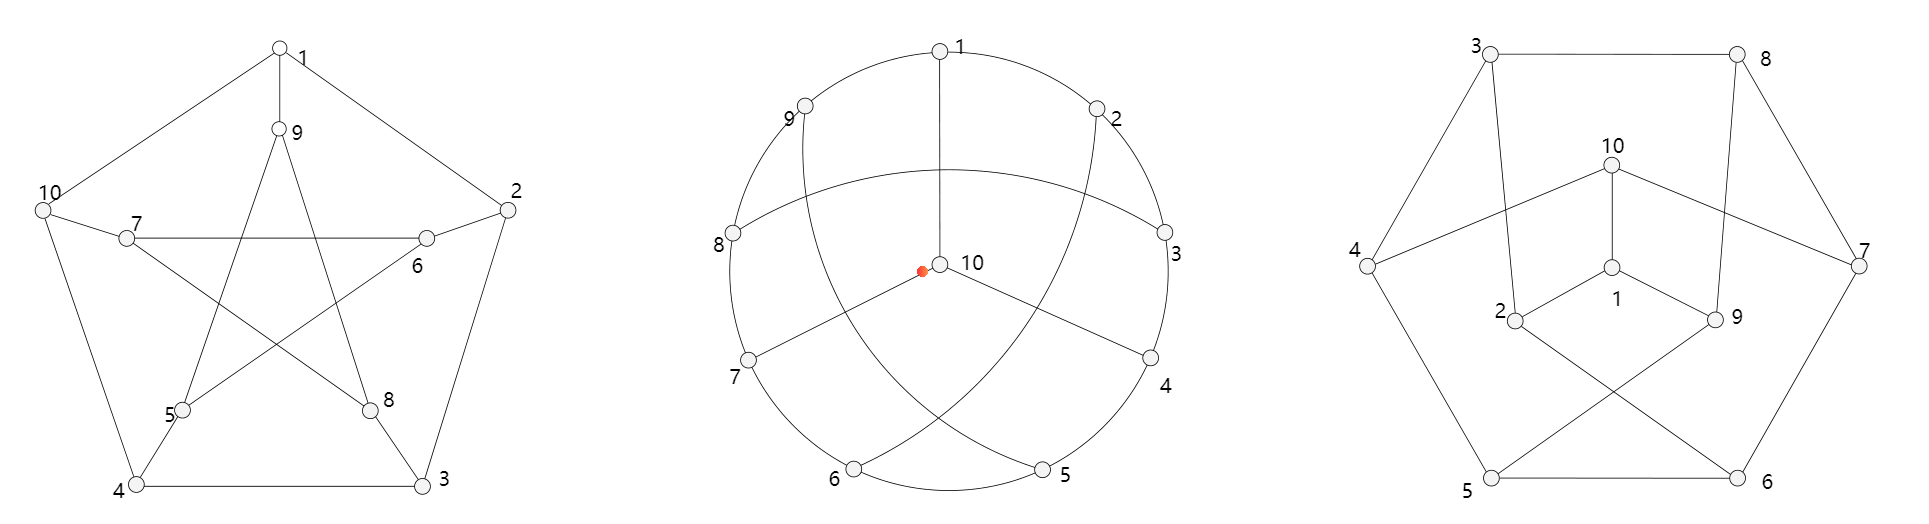
\includegraphics[scale=0.27]{PetersonGraphIsom.png}

它们的边均有且仅有:从1到9的9-圈,边2-6,边3-8,边4-10,边5-9,边7-10.这些构成了所有15条边,从而可以看出它们确实互相同构.
\end{proof}

\paragraph{1.3.15a de Bruijn-Erd\"os 定理}$G[X, Y]$是二部图,其每个顶点都与另一个部分中至少一个(但不是全部)顶点连接,若$\forall xy\notin E$有$d(x)\geq d(y)$,证明$\abs{Y}\geq \abs{X}$,取等当且仅当$\forall xy\notin E, d(x)=d(y)$.
\begin{proof}
由于有
$$\abs{X}=\sum_{x\in X}\sum_{\substack{y\in Y\\ xy\notin E}}\frac{1}{\abs{Y}-d(x)}, \abs{Y}=\sum_{y\in Y}\sum_{\substack{x\in X\\ xy\notin E}}\frac{1}{\abs{X}-d(y)}$$
若$\abs{Y}<\abs{X}$,则对$\forall xy\notin E$有$\abs{X}d(x)>\abs{Y}d(y)$,从而有
$$1=\sum_{\substack{x\in X, y\in Y\\ xy\notin E}}\frac{1}{\abs{X}(\abs{Y}-d(x))}>\sum_{\substack{x\in X, y\in Y\\ xy\notin E}}\frac{1}{\abs{Y}(\abs{X}-d(y))}=1$$
矛盾,因此$\abs{Y}\geq \abs{X}$.考虑取等条件,若$\abs{X}=\abs{Y}$且有$x_0y_0\notin E, d(x_0)>d(y_0)$,则
$$\abs{X}=\sum_{\substack{x\in X, y\in Y\\ xy\notin E}}\frac{1}{\abs{X}-d(x)}>\sum_{\substack{x\in X, y\in Y\\ xy\notin E}}\frac{1}{\abs{Y}-d(y)}=\abs{Y}$$
矛盾,从而可见若能取到$\abs{X}=\abs{Y}$则$\forall xy\notin E$有$d(x)=d(y)$,反之若已有$\forall xy\notin E, d(x)=d(y)$,而
$$1=\sum_{\substack{x\in X, y\in Y\\ xy\notin E}}\frac{1}{\abs{X}\abs{Y}-\abs{X}d(x)}=\sum_{\substack{x\in X, y\in Y\\ xy\notin E}}\frac{1}{\abs{Y}\abs{X}-\abs{Y}d(y)}=1$$
则可见$\abs{X}=\abs{Y}$,从而可知取等条件有且仅有$\forall xy\notin E, d(x)=d(y)$.
\end{proof}

\section{第二章\; 子图}
\paragraph{2.1.5}(1)若简单图$G$有$\delta\geq 2$,则其中含长度$\geq \delta+1$的圈.(2)对每个$k\geq 2$给出简单图$G$,其满足$\delta=k$但不含任何长度$>k+1$的圈.
\begin{proof}
(1)任选图中一个顶点$v_1$,其至少与$\delta$个顶点相邻,任取其一记为$v_2$,$v_2$至少与$\delta-1$个未选择顶点相邻.以此类推,可得长$\delta$的路$v_1v_2\cdots v_{\delta+1}$.若$v_{\delta+1}$与$v_1$相邻则命题成立,否则$v_{\delta+1}$与已选择的$\delta$个顶点中至多$\delta-1$个相邻,从而有未取到的新点$v_{\delta+2}\notin \cbr{v_i}_{i=1}^{\delta+1}$.继续考虑$v_{\delta+2}$是否与$v_1,v_2$其中的点相邻,若否则同理可取到$v_{\delta+3}$.以此类推,总有$v_{\delta+k}$不与$\cbr{v_i}_{i=1}^{k}$中的点相邻,而$k=n-\delta$时必然有$\cbr{v_i}_{i=1}^{k}$中的点与$v_n$相邻,因此这一算法能在有限步后终止,即总能取到长至少$\delta+1$的圈.

(2)考虑完全图$K_n$,则$\delta=n-1$,而图中圈长不超过$n$.
\end{proof}

\paragraph{2.2.4}用最长路径的论证给出定理2.3的证明.
\begin{quote}
    \textbf{定理2.3 R\'edei定理}: 每个竞赛图都有有向Hamilton圈.
\end{quote}
\begin{proof}
考虑竞赛图$G$中的最长路$v_1\cdots v_k$,若有$v\in V-\cbr{v_i}_{i=1}^k$,则$(v_1,v),(v,v_k)\in E$,否则与最长条件矛盾.考虑使$(v_i,v)\in E$的下标最大的$v_i$,有$1\leq i\leq k-1$,则仍有$(v,v_{i+1})\in E$,从而有更长的路$v_1\cdots v_i v v_{i+1}\cdots v_k$,矛盾,从而最长路遍历所有顶点,即为Hamilton路.
\end{proof}

\paragraph{2.3.1}(1)$\forall e\in E$证明$c(G/e)=c(G)$.(2)$G$是无圈图,$e\in E$,证明(i)$G/e$是无圈图.(ii)$m=n-c$.
\begin{proof}
(1)若$G$是连通图,记$e=u_1 u_2\in E$,其在$G/e$中缩并为顶点$v$.在$V(G)-\cbr{u_1,u_2}$中任取两顶点$s,t$,则在$G$中有路$sv_1\cdots v_k t$连接之.若路中不含$u_1,u_2$,则在$G/e$中仍有同样的路连接$s$和$t$;若路中有$v_i=u_1$或$u_2$,则$sv_1\cdots v_{i-1}vv_{i+1}\cdots v_k t$为$G/e$中连接$s$与$t$的路.由$s,t$选取的任意性可知$G/e$是连通的.

现考虑任意图$G,c(G)=k$,则有$G=G_1+\cdots +G_k$,其中$G_i(i\in [k])$为其所有连通分支.若$e$是其中$G_i$的边,则$G/e=G_1+\cdots +G_i/e+\cdots +G_k$,由$G_i/e$仍为连通图可知$c(G/e)=k$,从而得证.

(2.1)仍记$e=u_1 u_2\in E$在$G/e$中缩并为顶点$v$.若$G/e$中有不经过$v$的圈$v_1v_2\cdots v_kv_1$,则在$G$中同样存在该圈,矛盾.若有经过$v$的圈$vv_1\cdots v_k v$,则在$G$中$v_1$与$v_k$均至少与$u_1,u_2$其中一个相邻,从而在$G$中同样存在圈,矛盾.综上可知$G/e$同样为无圈图.

(2.2)收缩无圈图$G$中的任意边$e$时,由上知$c(G)=c(G/e)$,由无圈图无自环知$v(G/e)=n-1$,由无圈图无平行边知$e(G/e)=m-1$.而无圈图收缩后仍为无圈图,从而可以对所有边不断收缩$m$次直到无边(即平凡图),此时其顶点数等于连通分支个数$c$.从而
$$\begin{aligned}
        c & =v(G/\cbr{e_1,\cdots,e_m})-e(G/\cbr{e_1,\cdots,e_m})=[v(G/\cbr{e_1,\cdots,e_{m-1}})-1]-[e(G/\cbr{e_1,\cdots,e_{m-1}})-1] \\
          & =v(G/\cbr{e_1,\cdots,e_{m-1}})-e(G/\cbr{e_1,\cdots,e_{m-1}})=\cdots                                                      \\
          & =v(G/e_1)-e(G/e_1)=[v(G)-1]-[e(G)-1]                                                                                     \\
          & =n-m
    \end{aligned}$$
从而得证.
\end{proof}

\paragraph{2.4.2 偶有向图}称有向图$D$是偶图,若$\forall v\in V, d^-(v)=d^+(v)$.证明Veblen定理的有向图版本:有向图有有向圈分解$\iff$有向图是偶图.
\begin{proof}
$\implies:$若$G$有一个圈分解$\cbr{G_1,\cdots,G_k}$,即顶点$v$在$G_i$中的度数为$d^-_i(v)$与$d^+_i(v)$,则每个$G_i$中不在圈上的顶点$v$有$d_i^-(v)=d_i^+(v)=0$,在圈上的则有$d^-(v)=d^+(v)=1$,从而$$\forall v\in V, d^-(v)=\sum_{i=1}^k d^-_i(v)=\sum_{i=1}^k d^+_i(v)=d^+(v).$$

$\impliedby:$对$m$进行归纳,当$m=0$时有空的圈分解,下设$m<M$时命题成立,考虑$m=M$的情形.由于任意非孤立点$v$有$d^+(v)=d^-(v)\geq 1$,故可任取非孤立点$v_1, d^+(v_1)\geq 1$,故$v_1$至少有一条出边$(v_1,v_2)$,再对$v_2$如此考虑,以此类推.若有$v_k$使得某个$1\leq i\leq k-1$有$v_k=v_i$,则有有向圈$C=(v_i,v_{i+1},\cdots,v_k,v_i)$.若对$\forall k\geq 1$都没有对应的$v_i$,则其矛盾于图的有限性,故总有有向圈$C$.

考虑$G$的删边子图$G-C=(V,E-C)$,由前知$\forall v\in V, d^+_C(v)=d^-_C(v)$,从而$d^+_{G-C}(v)=d^+_G(v)-d^+_C(v)=d^-_G(v)-d^-_C(v)=d^-_{G-C}(v)$,且$e(G-C)<e(G)=M$,故满足归纳假设,即$G-C$已存在圈分解$\cbr{C_1,\cdots,C_k}$,从而$G$也有圈分解$\cbr{C_1,\cdots,C_k,C}$.
\end{proof}

\paragraph{2.5.1}(1)证明定理2.9.(2)证明命题2.13.(3)由命题2.11推出定理2.14.
\begin{quote}
    \textbf{定理2.9}:图$G$及其顶点子集$X\subset V$有$d(X)=\sum_{v\in V}d(v)-2e(X)$.

    \textbf{命题2.11}:图$G$及其顶点子集$X,Y\subset V$有$\partial(X)\triangle\partial(Y)=\partial(X\triangle Y)$.

    \textbf{命题2.13}:$F_1,F_2$是$G$的生成子图,$X\subset V$是顶点子集,则$\partial_{F_1\triangle F_2}(X)=\partial_{F_1}(X)\triangle\partial_{F_2}(X)$.

    \textbf{定理2.14}:图的一个边子集是边割集当且仅当其是键的不交并.
\end{quote}

\begin{proof}
(1)定理2.9的证明:
$$\begin{gathered}
        d(X)=\#\cbr{xy\in E|x\in X, y\in V-X}=\sum_{x\in X}\sum_{\substack{y\in V-X\\ xy\in E}}1=\sum_{x\in X}\br{\sum_{\substack{y\in V\\ xy\in E}}1-\sum_{\substack{x'\in X\\ xx'\in E}}1}=\sum_{x\in X}d(x)-\sum_{x\in X}\sum_{\substack{x'\in X\\ xx'\in E}}1\\
        \sum_{x\in X}\sum_{\substack{x'\in X\\ xx'\in E}}1=\sum_{(x,x')\in X^2}\sum_{xx'\in E}1=2\sum_{x,x'\in X}\sum_{xx'\in E}1=2e(X)
    \end{gathered}$$

(2)推论2.13的证明:
$$\begin{aligned}
        \partial_{F_1\triangle F_2}(X) & =\cbr{xy\in E(F_1\triangle F_2)|x\in X, y\in V-X}=\cbr{xy\in E(F_1)\triangle E(F_2)|x\in X, y\in V-X}                          \\
                                       & =\cbr{xy\in E(F_1)|x\in X, y\in V-X}\triangle \cbr{xy\in E(F_2)|x\in X, y\in V-X}=\partial_{F_1}(X)\triangle \partial_{F_2}(X)
    \end{aligned}$$

(3)定理2.14的证明:$\implies:$若$S\subset E$是一个边割集,则要么$S$是键,要么不是.若是则证毕,否则由$S$不是极小边割集知,有键$B_1\subsetneq S$,且$S-B_1=S\triangle B_1$是边割集.继续考虑$S-B_1$是不是键,以此类推.由$S$是有限集可知,总存在$n\geq 1$使得$S-\bigcup_{1\leq i< n}B_i$是键,而由上构造键$B_i$之间两两不交,从而可取到不交并$S=\bigsqcup_{1\leq i\leq n}B_i$.

$\impliedby:$若$S=\bigsqcup_{1\leq i\leq n}B_i$,其中$B_i$是键且其间两两不交,则$B_1\sqcup B_2=B_1\triangle B_2$是边割集,$B_1\sqcup B_2\sqcup B_3$同理也是,以此类推$S$是边割集.
\end{proof}

\paragraph{2.5.4}$G$是无自环图,$X,Y\subset Y$.(1)证明
$$d(X)+d(Y)=d(X\cup Y)+d(X\cap Y)+2e(X-Y,Y-X)$$
(2)推出关于顶点子集度数的次模不等式
$$d(X)+d(Y)\geq d(X\cup Y)+d(X\cap Y)$$
(3)叙述并证明有向图版本的次模不等式.
\begin{proof}
(1)(2)下记$C=V-(X\cup Y)$,有分解
$$\begin{aligned}
        d(X)+d(Y)= & \bbr{e(X-Y,C)+e(X\cap Y,C)+e(X-Y,Y-X)+e(X\cap Y,Y-X)}                                  \\
                   & +\bbr{e(Y-X,C)+e(X\cap Y,C)+e(Y-X,X-Y)+e(X\cap Y,X-Y)}                                 \\
        =          & \bbr{e(X-Y,C)+e(X\cap Y,C)+e(Y-X,C)}+\bbr{e(X\cap Y, X-Y)+e(X\cap Y,Y-X)+e(X\cap Y,C)} \\
                   & +\bbr{e(X-Y,Y-X)+e(Y-X,X-Y)}                                                           \\
        =          & d(X\cup Y)+d(X\cap Y)+2e(X-Y,Y-X)\geq d(X\cup Y)+d(X\cap Y)
    \end{aligned}$$
(3)对于有向图,同上证明也有
$$d^+(X)+d^-(Y)=d^+(X\cup Y)+d^+(X\cap Y)+a(X-Y,Y-X)+a(Y-X,X-Y)\geq d^+(X\cup Y)+d^+(X\cap Y)$$
\end{proof}

\paragraph{2.5.5}奇图即每个顶点度数为奇数的图.证明$G$是奇图$\iff \forall X\subset V, d(X)\equiv\abs{X}\bmod 2$.

\begin{proof}
$\implies:$注意到对于奇图总有$d(v)\equiv 1\bmod 2 (\forall v\in V)$,从而有
$$d(X)=\sum_{x\in X}d(x)-2e(X)\equiv \sum_{x\in X}d(x)\equiv \sum_{x\in X}1=\abs{X}\pmod 2$$
$\impliedby: d(v)=d(\cbr{v})\equiv \abs{\cbr{v}}=1\pmod 2$,由$v$选取的任意性知为奇图.
\end{proof}

\paragraph{2.6.2}证明边空间$\mathcal{E}(G)$是关于对称差运算的$\F_2$-向量空间,且同构于$\F_2^E$.

\begin{proof}
由定义$\mathcal{E}(G)=2^{E}$,考虑映射$\varphi:\mathcal{E}(G)\to \mathbb{F}_2^E, S\mapsto (\mathbf{f}_S: e\mapsto [e\in S])$,其中$[e\in S]$是Iverson括号,下考虑$\mathbb{F}_2^E$中由逐点运算自然诱导的$\mathbb{F}_2$-向量空间结构,为同样赋予$2^E$以$\mathbb{F}_2$-向量空间结构,定义$0\cdot S=\varnothing, 1\cdot S=S$.由$\varphi(S_1\triangle S_2)=\mathbf{f}_{S_1\triangle S_2}$和$\mathbf{f}_{S_1\triangle S_2}(e)=[e\in S_1\triangle S_2]=[e\in S_1]+[e\in S_2]$(此处加法是$\mathbb{F}_2$意义下的),从而知$\mathbf{f}_{S_1\triangle S_2}=\mathbf{f}_{S_1}+\mathbf{f}_{S_2}$.另一方面$0\cdot \mathbf{f}_S=\mathbf{0}=\mathbf{f}_{\varnothing}, 1\cdot \mathbf{f}_S=\mathbf{f}_S$.综上有
$$\forall S_1,S_2\in \mathcal{E}(G),\forall a\in \mathbb{F}_2, \varphi(S_1\triangle S_2)=\varphi(S_1)+\varphi(S_2), \varphi(aS_1)=a\varphi(S_1)$$
从而$\varphi$是一个$\mathbb{F}_2$-模同态,而由上同理$\mathbf{f}_S\mapsto S$为$\varphi$的一个逆映射和$\mathbb{F}_2$-模同态,从而$\varphi$为同构.
\end{proof}

\section{第三章\; 连通图}
\paragraph{3.1.3}证明由顶点间连通关系决定的等价类就是图连通分支的顶点集.
\begin{proof}
考虑顶点关于连通关系的任意等价类$[a]=\cbr{v\in V|\text{存在}av\text{-途径}}$,则$\forall v\in [a], a$与$v$在同一个连通分支,即$[a]$在某个连通分支内.若某个连通分支中有多个等价类$[a],[b]$,则由$a,b$在同一个连通分支中知有从$a$到$b$的路径,从而$a,b$同属一个等价类,矛盾.综上可知,连通等价类即连通分支.
\end{proof}

\paragraph{3.1.8}$G$是直径为2的简单图,$\Delta=n-2$,证明$m\geq 2n-4$.
\begin{proof}
考虑度数为$n-2$的顶点$u$,其与顶点$v_1,\cdots,v_{n-2}$相邻,且有唯一顶点$v$与之不相邻.考虑删点子图$G-\cbr{u,v}$所有连通分支的顶点集$V_1,\cdots,V_k (1\leq k\leq n-2)$,若有$V_i$使得$v$与$V_i$间无边,则连接$v$与$V_i$的路径必然首先经过某个$V_j(j\neq i)$,否则$v$与$V-v$不连通,而又知$V_i$与$V_j$间不连通知其次只能经过$u$,最后从$u$到$V_i$,从而$d(v,V_i)\geq 3$,与题设矛盾.因此$v$与每个$V_i$之间都有边.

综上所述,$u$与除$v$外的所有顶点相邻,$v$与每个$V_i$中至少一个顶点相邻,而$V_i$之间两两无边,从而$E=E(u)\sqcup E(v)\sqcup E(V_1)\sqcup \cdots \sqcup E(V_k)$,注意到作为连通分支,$E(V_i)=E(V_i,V_i)\geq \abs{V_i}-1$.从而
$$m=d(u)+d(v)+\sum_{i=1}^k e(V_i)\geq n-2+\sum_{i=1}^k 1+\sum_{i=1}^k (\abs{V_i}-1)=n-2+\abs{\bigsqcup_{i=1}^k V_i}=2n-4$$
\end{proof}

\paragraph{3.2.3}$G$是连通偶图,证明(1)$G$没有割边.(2)$\forall v\in V, c(G-v)\leq d(v)/2$.
\begin{proof}
$G$作为偶图有圈分解$G=\bigcup_{i\in [k]}C_i$,从而$G$中任意边$e$都在某条圈$C_i$中,由推论3.3.2知其等价于$e$不是割边(cut edge).对于任意顶点$v$,若其是某条圈$C_i$的顶点,则$d_{C_i}(v)=2$,而$\cbr{C_i}_{i=1}^k$之间边两两不交,从而$d(v)=\sum_{i=1}^k d_{C_i}(v)=\sum_{v\in V(C_i)}2$,即圈分解$\cbr{C_i}_{i=1}^k$中有$d(v)/2$条圈以$v$作为顶点.从$G$中依次删除$v$在$C_i(i\in [k])$中的边,直到使$v$成为孤立点.由于仅删除$v$在$C_i$中连接的一条边不会产生新的连通分支,故删去全部两条仅可能增加一个连通分支,从而对$d(v)/2$条圈如此操作后最多增加$d(v)/2$个连通分支.最后删去连通分支$v$,从而$c(G-v)\leq (1+d(v)/2)-1=d(v)/2$.
\end{proof}

\paragraph{3.3.3}图$G$中有两不同顶点$x,y$,令$G+e$是向$G$中添加连接$x,y$的边得到的图.(1)证明$G$有连接$x,y$的Euler迹$\iff G+e$有Euler回路.(2)证明$G$有连接$x,y$的Euler迹$\iff d(x),d(y)$为奇数且$\forall v\in V-\cbr{x,y}, d(v)$是偶数.
\begin{proof}
(1)若在$G$中存在连接$x$和$y$的Euler迹$x e_1 v_1\cdots v_k e_m y$,即迹中的$e_1,\cdots,e_m$为$G$中全部边,则在$G+e$中可取Euler回路$x e_1 \cdots e_m y e x$,其边已经遍历了$G+e$中全部边.反之若能在$G+e$中取到上述Euler回路,去掉$e$即为$G$中连接$x$和$y$的Euler迹,因为已经遍历了所有$G$中的边.

(2)若$G$中存在连接$x$和$y$的Euler迹,则$G+e$中含Euler回路,从而是连通偶图,即$G$中除$x,y$的顶点度数为偶数,$x,y$的度数为奇数.反之,由题设可知$G+e$中含Euler回路,即$G$中存在连接$x$和$y$的Euler迹.
\end{proof}

\paragraph{3.3.4}$G$是连通图,$X$是$G$中奇数度数的顶点构成的集合.设$\abs{X}=2k, k\geq 1$.(1)证明$G$中有$k$条边不交的迹$Q_1,Q_2,\cdots,Q_k$使得$E(G)=\bigsqcup_{i=1}^k E(Q_i)$. (2)推出$G$中含$k$条边不交的迹将$X$中的点成对连接.
\begin{proof}
对于$X=\cbr{x_1,\cdots,x_{2k}}$,给$G$中加$k$条边$E'=\cbr{x_1x_2,x_3x_4,\cdots,x_{2k-1}x_{2k}}$,则加边图$G+E'$中每个顶点的度数为偶数,从而为连通偶图,即存在Euler回路,其经过所有$E'$的$k$条边.将圈中所有$E'$中的边删去,则可断为相应的$k$条迹,每条连接$X$中的两个顶点,且所有迹中边不交,并集仍为$E(G)$.
\end{proof}

\paragraph{3.3.6 支配子图}$G$的子图$F$是支配子图,若$G$中任意边都有至少一个端点在$F$中.令$m\geq 3$,证明$L(G)$是Hamilton图$\iff G$有支配Euler子图.
\begin{proof}
简单图$G$的线图$L(G)$以$E(G)=\cbr{e_i}_{i=1}^m$为顶点,在$L(G)$中存在边$e_ie_j$等价于$G$中$e_i$与$e_j$有共同顶点$v$.任取$v_i\in V(G)$,在所有$d(v_i)$条连接$v_i$的边中任取两条,其在$L(G)$中有边相连,从而$v_i$对应于$E(L(G))$中的$m_i=\binom{d(v_i)}{2}$条边,记这些边为$v_{i1},\cdots, v_{im_i}$,即$E(L(G))=\cbr{v_{ij}|i\in [n], j\in [m_i]}$.

$\implies:$考虑$L(G)$中的Hamilton圈$e_1 v_{1j_1} e_2 \cdots e_m v_{mj_m} e_1$,则取$\cbr{v_1,\cdots,v_m}$为$G$子图$F$的顶点集(其中可能有$v_i=v_j, i\neq j$).由于$L(G)$中任意点$e_i$都与某边$v_{ij_i}$相邻,从而$G$的任意边$e_i$都与$F$的顶点$v_i$相邻,即$F$是支配子图.下为$F$添加边使其成为Euler图.

考虑$G$的点边交错的循环序列$R=(e_1, v_1, e_2, \cdots, e_m, v_m)$,若其中存在子序列$(v_k, e_{k+1}, v_k=v_{k+1}, e_{k+2}, \cdots,\linebreak e_{\ell-1}, v_k=v_\ell)$,则将该子序列替换为$(v_k)$,如此替换直到不能继续.注意到每次替换前后,序列中所有点仍为$E(F)$,任意子序列$(e_i,v_j,e_k)$都表明$G$中$v_j$与$e_i,e_k$相连.操作后得到序列$R_0=(e_{i_1}, v_{i_1}, \cdots, e_{i_\ell}, v_{i_\ell})$,令$E(F)=\cbr{e_{i_1},\cdots,e_{i_\ell}}$.若$R=(v),E(F)=\varnothing$,命题得证.否则由于$\forall v\in E(F)$都在$R_0$中有一些形如$(e_i, v_k, e_j)$的不相邻子序列,从而$v_k$与偶数条边相连,即$F$为偶图.最后,$F$中任意两点$v_i,v_j$,都可以在$R_0$中取到子序列$(v_i, e_{i_i}, \cdots, e_{i_j}, v_j)$,这对应于$F$中的一条路径,故$F$也是连通的.综上,$F$即为所需的支配Euler子图.

$\impliedby:$若$F$是$G$的一个支配Euler子图,则$F$中存在Euler回路$v_1 e_1\cdots e_{k-1} v_k e_k v_1$,其对应于$L(G)$中的圈$C=e_1 v_{2j_2}\cdots v_{kj_k} e_k v_{1j_1} e_1$.若$e\in E(G)$不在圈上,则由$F$是支配子图知有$v_i\in V(F)$与其相连,从而其与$e_{i-1},e_i$均有公共端点$v_i$,从而可以向$C$中添加边,即为$e_1 \cdots e_{i-1} v_{ij_a} e v_{ij_b} e_{i+1} \cdots e_1$.对所有不在圈上的边如此操作,最终可得到$L(G)$中的经过所有顶点恰一次的回路$C'=e_1 \cdots e_m v_{1j_1} e_1$.若其中有边相同,即说明有点被经过超过一次,矛盾.从而$C'$是$L(G)$的Hamilton圈.
\end{proof}

\section{第四章\; 树}
\paragraph{4.1.1}(1)若树有$\Delta=k$,则至少有$k$个叶子.(2)什么样的树有恰好$k$个叶子?
\begin{proof}
若$\Delta(T)=k$,取树中度数为$k$的节点$v$并以其为根节点,即$v$有$k$个子节点.而每个子节点及其子节点形成的子树叶子数至少为1,从而$T$的叶子数至少为$k$.$K_{1,k}$即为恰有$k$个叶子的树.
\end{proof}

\paragraph{4.2.1}连通图$G$有边$e$.(1)在$G$的含$e$生成树集合与$G/e$的生成树集合间构造双射.(2)推出命题4.9.
\begin{proof}
取任意边$e_0=xy\in E(G)$,注意到有满射(从而为双射)$f:E(G)-\cbr{e_0}\to E(G/e_0)$,从而可考虑映射
$$\varphi:\cbr{G 中含 e_0 的生成树 T}\to \cbr{ G/e_0 的生成树 T'}, T=(V(G),E(T))\mapsto T'=(V(G/e_0),E(T')=f(E(T))).$$
由于$f$是双射,从而$E(T)\to E(T'), e\mapsto f(e)$也是双射,故可取逆映射
$$\varphi\rev: T'=(V(G/e_0),E(T'))\mapsto T=(V(G),E(T)=f\rev(E(T'))),$$
从而$\varphi$是双射.最后,$G$的生成树数量等于含$e_0$与不含$e_0$的生成树数之和,从而有$t(G)=t(G-e_0)+t(G/e_0)$.
\end{proof}

\paragraph{3.4.11*}(1)证明含奇长度有向闭途径的有向图含有向奇圈.(2)证明含奇圈的强有向图含有向奇圈.
\begin{proof}
(1)有向图$D$中存在奇长度有向闭途径$W=(v_1,a_1,\cdots,a_k,v_1)$,若其中所有顶点$v_i$互不相同则命题成立,否则考虑其中相同顶点$v_i=v_j(i<j)$,则$W$可以拆为两个子途径$W_1=(v_1,a_1,\cdots,v_i,a_j,\cdots,a_k,v_1)$与$W_2=(v_i,a_i,\cdots,a_{j-1},v_j)$.对子途径如此不断拆分直到其中所有顶点都互不相同(即成为圈),则$W$可视作圈$W_1,\cdots,W_\ell$首尾相连,而所有圈$W_i$长度之和,即$W$长度为奇数,故存在圈$W_k$长度为奇数,即得证.

(2)强有向图$D$的底图$G(D)$中有奇圈$v_1 a_1 \cdots a_k v_1$,考虑$W_i$为$D$中极小$(v_i,v_{i+1})$-途径$(i\in [k])$,若已有弧$a_i=(v_i,v_{i+1})$则$W_i=(v_i,a_i,v_{i+1})$,若否则由底图中存在圈知存在$(v_{i+1},v_i)$-途径$(v_{i+1},a_i,v_i)$,从而由强连通性知存在极小$(v_i,v_{i+1})$-途径$W_i$.若$W_i$长为偶数,则$W_i$后加上$(v_{i+1},a_i,v_i)$成为有向奇圈,命题成立.若否,则综上所述可知所有有向途径$W_1,\cdots,W_k$长度为奇数,故将其首尾相连得到的闭途径$W$长也为奇数,由(1)知其中存在有向奇圈,从而得证.
\end{proof}

\paragraph{4.2.8}使用定理4.11与习题3.4.11b,证明有向图含有向奇圈等价于其中一些强连通分支不是二部图.
\begin{proof}
    $\implies:$有向图$D$有有向奇圈则其底图$G(D)$有奇圈,从而$G(D)$不是二部图,故$D$也不是.$\impliedby:$若$D$的某些强连通分支不是二部图,则该强连通分支的底图中存在奇圈,由习题3.4.11(2)知$D$中存在有向奇圈.
\end{proof}

\paragraph{4.3.5}证明定理4.13,推论4.14与4.15.
\begin{proof}
    (1)定理4.13的证明:由于基本键(fundamental bond)$B_e$是边割集,因此其对称差$B=\underset{e\in S}{\triangle}B_e$也是边割集,而由$e\in B_e\subset \overline{T}\cup\cbr{e}$可知$B_e\cap T=\cbr{e}$,从而
    $$B\cap T=\br{\underset{e\in S}{\triangle}B_e}\cap T=\underset{e\in S}{\triangle}(B_e\cap T)=\underset{e\in S}{\triangle}\cbr{e}=S$$
    最后,若$G$中有另一边割集$B'$满足$B'\cap T=S$,则$$(B\triangle B')\cap T=(B\cap T)\triangle (B'\cap T)=S\triangle S=\varnothing$$
    从而边割集$B\triangle B'$含于$\overline{T}$中,而$\overline{T}$中仅有的边割集为$\varnothing$,从而$B\triangle B'=\varnothing, B=B'$.

    (2)推论4.14的证明:对$G$中任意边割集$B$,考虑$S=B\cap T\subset T$,由上定理知满足$S=B'\cap T$的边割集$B'$仅有$B'=B=\underset{e\in S}{\triangle}B_e$,从而任意边割集均为一些基本键的对称差.

    (3)推论4.15的证明:在定理4.13中取$S=T$,则$B=\underset{e\in T}{\triangle}B_e, B\cap T=T$,即$T\subset B$,且$B$是唯一的.
\end{proof}

\paragraph{4.3.10}证明任意含两个边不交的生成树的图中含:(1)一个Euler生成子图;(2)两个偶子图构成的覆盖.
\begin{proof}
    考虑图$G$中两个边不交的生成树$T_1,T_2$,有$T_2\subset \overline{T_1}\subset C_2$,其中$C_2$是唯一包含$\overline{T_1}$的偶子图,从而$C_2$同样含所有顶点(即生成子图)且连通,故$C_2$为Euler生成子图.同理可取出$C_1$,故$E=T_1\cup \overline{T_1}\subset C_1\cup C_2$,即$\cbr{C_1,C_2}$为所求覆盖.
\end{proof}

\paragraph{6.1.1}$T$是连通图$G$的BFS树,证明$\ell(v)=d_T(r,v),\forall v\in V$.
\begin{proof}
$r$是$T$的根节点,从而$\forall v\in V$在$T$中有且仅有一个顶点$v_1$与之相连,且$\ell(v_1)=\ell(v)-1$,以此类推可知存在长$\ell(v)$的$vr$-路径$vv_1v_2\cdots v_{\ell(v)-1}r$,该路径在$T$中唯一,从而得证.
\end{proof}

\section{第五章\; 不可分图}
\paragraph{5.1.2}连通图$G(n\geq 3)$中有割边$e=uv$,证明$u$或$v$是$G$的割点.
\begin{proof}
由$e$是割边知$G-e$不连通,且$u$与$v$分属两个连通分支.由$n\geq 3$知另有点$w$与$u$或$v$同连通分支.设$w$与$u$同连通分支,若$G-u$中有连接$w$与$v$的路,则在$G-e$中有同样的路,矛盾,故在$G-u$中$w$与$v$不在同一连通分支,即$G-u$不连通,$u$是割点.同理可对$v$讨论,故$u,v$中至少一个为割点.
\end{proof}

\paragraph{5.2.2}图$G$中有边$e$,证明:(1)若$G-e$是不可分图且$e$不是$G$中的自环,则$G$也是不可分图;(2)若$G/e$是不可分图且$e$不是$G$中的自环或割边,则$G$也是不可分图.
\begin{proof}
(1)$G-e$不可分故为连通无自环图,而$e$不是自环,故$G$也为连通无自环图,仅需证$G$无割点.记$e=uv$,由$G-e$中无割点知$(G-e)-u=G-u$和$(G-e)-v=G-v$均连通,且$\forall w\in V-\cbr{u,v}$有$(G-e)-w$连通,从而加边$e$得到的$G-w$仍连通,故$u,v,w$均不是割点,即$G$无割点.

(2)记$e=uv$,由$G/e$不可分知其连通且无自环,从而$G$同样连通且无自环.而若$G$有除$u,v$外的割点,则其也为$G/e$的割点,矛盾.若$G$的割点为$u$或$v$,即$G-u$或$G-v$不连通,则$G/e$删去$u,v$缩并而成的顶点同样不连通,矛盾于$G/e$不可分.从而$G$不可分.
\end{proof}

\paragraph{5.2.9}考虑定理5.4的证明中出现的图$G'$,证明(1)$G'$连通;(2)$G'$中每条边都在一个圈上.
\begin{proof}
对于不可分图$G$中顶点$v$,其是$H=G-f$的割点且满足$d(v)\geq 4, \abs{N(v)}\geq 2$.在$H$中$v$连接分别属于两个不同区块的边$e_1=vv_1, e_2=vv_2$,将两者分拆(split off),即在$H$中删去$e_1,e_2$并加边$e=v_1v_2$,即得$G'$.由$d(v)\geq 4$知$G'$中仍有连接$v$的边$e'$.

由$H$区块树为路径,知$v$仅连接两个区块,从而$H-v$仅被分为两个连通分支,$x,y$分别在两分支中,则$(H-v)+e$连通,$G'$同样连通.而由定理5.4知$G'$无割边,由命题3.2知$G'$中每条边都在一个圈上.
\end{proof}

\paragraph{5.2.11}不可分图$G$中有边$e$使得$G-e$可分,证明$G-e$的区块树是路.
\begin{proof}
$e=xy$的端点$x,y$是$G-e$的分离点或某区块的内部顶点,其不能是同一个区块$B$的两内部顶点,否则$B+e$仍是$G=(G-e)+e$中的区块,与$G$不可分矛盾.从而$x,y$对应于区块树$B(G-e)$的两节点,其在树上有唯一路径连接.对于任意不在路径上的区块,其在$G=(G-e)+e$中同样是区块,从而矛盾,即所有$B(G-e)$中区块都在路上.从而也可看出$e$端点分属$B(G-e)$的两叶子区块.
\end{proof}

\section{第九章\; 连通度}
\paragraph{9.1.3}(1)若简单图$G$满足$\delta\geq n-2$则$\kappa=\delta$.(2)对任意$n\geq 4$给出一个简单图$G$,使得$\kappa<\delta=n-3$.
\begin{proof}
    (1)若$G$中不存在一对不相邻点,即所有点两两相邻,则$G=K_n, \delta=\kappa=n-1$.若存在点$x,y$不相邻,则$n-2\leq\delta\leq d(x)\leq n-2$,从而$\delta=n-2$,对任意顶点至多有一个点与其不相邻.由于对任意不相邻点$x,y$,$N(x)=N(y)=V-\cbr{x,y}$,即$p(x,y)=n-2$,从而$\kappa(G)=\min_{u\neq v, uv\notin E}p(u,v)=n-2$,命题得证.

    (2)对$\forall n\geq 4$考虑$H=K_{n-2}-xy$,其中$x,y\in V(K_{n-2})$,显然$\delta(H)=\kappa(H)=n-4$.再在$H$中添加另外两点$u,v$,其与$V(K_{n-2})-\cbr{y}, V(K_{n-2})-\cbr{x}$中的$n-3$个点分别连接,得到$G$,显然$v(G)=n, \delta(G)=n-3$.令$S=V(K_{n-2})-\cbr{x,y}=V(G)-\cbr{x,y,u,v},\abs{S}=n-4$,由$G-S$不连通知$\kappa(G)\leq \abs{S}=n-4<\delta$.
\end{proof}

\paragraph{9.1.8}$G$是不完备的连通图,证明$G$是$k$-连通图$\iff \br{\forall u,v\in V, d(u,v)=2\implies p(u,v)\geq k}$.
\begin{proof}
    $\implies: \forall u,v\in V, p(u,v)\geq \kappa(G)\geq k$. $\impliedby:$若$G$不是$k$-连通图,取其极小点割集$S$,则$G-S$有连通分支$H_1,\cdots,H_r$.若在$G$中有$s\in S$与连通分支$H_i$不相邻,则$G-(S\cup\cbr{s})$中$H_i$仍是连通分支,这与$S$极小矛盾.因此$\forall s\in S$在两不同连通分支中分别有邻点$x,y$,显然两者不相邻,故$d(x,y)=2$且$S$是一个$xy$-点割,从而$\abs{S}<k\leq p(x,y)=c(x,y)\leq \abs{S}$,矛盾.
\end{proof}

\paragraph{9.1.10}(1)$G$是$k$-连通图,则$\forall e\in E, G/e$是$(k-1)$-连通图. (2)对每个$k\geq 4$找出一个$k$-连通图$G\neq K_{k+1}$,使得$\kappa(G/e)=k-1 (\forall e\in E)$.
\begin{proof}
    (1)$k$-连通即$\forall u,v\in V, p(u,v)\geq k$.记$e=xy$,则$\forall u,v\in V-\cbr{x,y}$有至少$k$条内点不交的$uv$-路,而$\cbr{x,y}$是其中最多2条的内点,故在$G/e$中$u,v$间仍有至少$k-1$条内点不交的路.而$u,v$中有一点为$x$或$y$,不失一般性取$u=x$,则$G$中$x,v$间的$k$条内点不交路同样为$G/e$中的.综上$p_{G/e}(u,v)\geq k-1$,从而得证.

    (2)考虑圈$C_{k+3}$的补图$\overline{C_{k+3}}$,即$K_{k+3}$去掉其中一个Hamilton圈所得的图.首先证明$\kappa(\overline{C_{k+3}})=k$:考虑$\overline{C_{k+3}}$中不相邻的点$u,v$,又记$u$与$u_0,v$不相邻,$v$与$v_0,u$不相邻,则$\forall w\in V-\cbr{u,v,u_0,v_0}, uwv$是$uv$-路且这$k-1$条路互不相交.再考虑路$uv_0u_0v$,其与上面的路不相交,从而$p(u,v)\geq k, k\leq\min_{u\neq v, uv\notin E}p(u,v)=\kappa\leq \delta=k$.而该图收缩任意边后总有点与另外两点不相邻,故$\delta(\overline{C_{k+3}}/e)=k-1\geq\kappa(\overline{C_{k+3}}/e)$,由(1)知$\kappa(\overline{C_{k+3}}/e)=k-1$.
\end{proof}

\paragraph{9.2.1}给出扇形引理(命题9.5)的证明.
\begin{proof}
    考虑$k$-连通图$G, x\in V, Y\subset V-\cbr{x}$是含$\geq k$点子集.在$G$外添加新点$z$,并将其与$Y$中所有点连接,得到图$H$.由引理9.3知$H$也是$k$-连通图,从而有$k$条内点不交的$xz$-路$P_1,\cdots,P_k$,每条$P_i$含有一条$(x,Y)$-路$Q_i$,由$P_i$之间内点不交知$Q_i$的内点与末端点不同,从而$Q_1,\cdots,Q_k$构成一个$x$到$Y$的$k$-扇.
\end{proof}

\paragraph{9.2.3}不可分图$G$中有圈$C, v(C)\geq 3$及顶点子集$S\subset V(C), \abs{S}=3$.若$G-V(C)$中有连通分支$H$与$S$的所有顶点相邻,则$\exists v\in H$到$S$有3-扇.
\begin{proof}
    记$S=\cbr{s_1,s_2,s_3}$,$H$中分别有点$h_1,h_2,h_3$与之相连.若有$v=h_1=h_2$,则在$H$中有$vh_3$-路$P$,故可取$vs_1, vs_2, vPh_3s_3$为3-扇.下考虑$h_1,h_2,h_3$互不相同,则$H$中有$h_1h_2$-路$P$,且有$(h_3,V(P))$-路$Q'$,$Q'$中可取到不与$P$相交的$(h_3,V(P))$-路$Q$,记$Q$末端点为$v$.则$v$分$P=h_1P_1vP_2h_2$,故有3-扇$vP_1h_1s_1, vP_2h_2s_2, vQh_3s_3$,显然它们内点不交.
    \footnote{这里并没有用到不可分与圈的条件.我不确定是否存在问题,或本就可如此.}
\end{proof}

\paragraph{9.3.2}(1)证明$\kappa\leq\kappa'\leq\delta$.(2)找出满足$\kappa=3,\kappa'=4,\delta=5$的图$G$.
\begin{proof}
    (1)任二点$u\neq v$间有$p'(u,v)$条边不交$uv$-路,但其并不一定内点不交,故$p'(u,v)\geq p(u,v)$.而以$v$为端点的$p'(u,v)$条边不交$uv$-路需要连接$v$的边数$d(v)\geq p'(u,v)$.综上有:
    $$\kappa=\min_{u\neq v}p(u,v)\leq \min_{u\neq v}p'(u,v)=\kappa'\leq \min_v d(v)=\delta$$
    
    (2)\href{https://mathworld.wolfram.com/OwensGraphs.html}{76点Owens图}满足条件.另可由\href{https://math.stackexchange.com/a/3389232/1046467}{此回答}思路构造图\footnote{也可以本质相同的思路构造类似满足要求的图,详见\href{https://math.stackexchange.com/a/5005649/1046467}{我的回答}
    }:考虑不交集合$V_1,V_2,\abs{V_1}=\abs{V_2}=5,V=V_1\sqcup V_2$为图顶点集.在$V_1,V_2$分别构造完备图$K_5$,并取子集$X\subset V_1, Y\subset V_2, \abs{X}=4, \abs{Y}=3$构造满射$f:X\to Y$,添加边$\cbr{\cbr{x,f(x)}|x\in X}$.最后取$x'\in X$与$x_0\in V_1-X$,以及$V_2-Y=\cbr{y_1,y_2}$,添加边$\cbr{x',x_0}$与$\cbr{y_1,y_2}$.如图,其满足$\kappa=3,\kappa'=4,\delta=5$:

    \begin{center}
        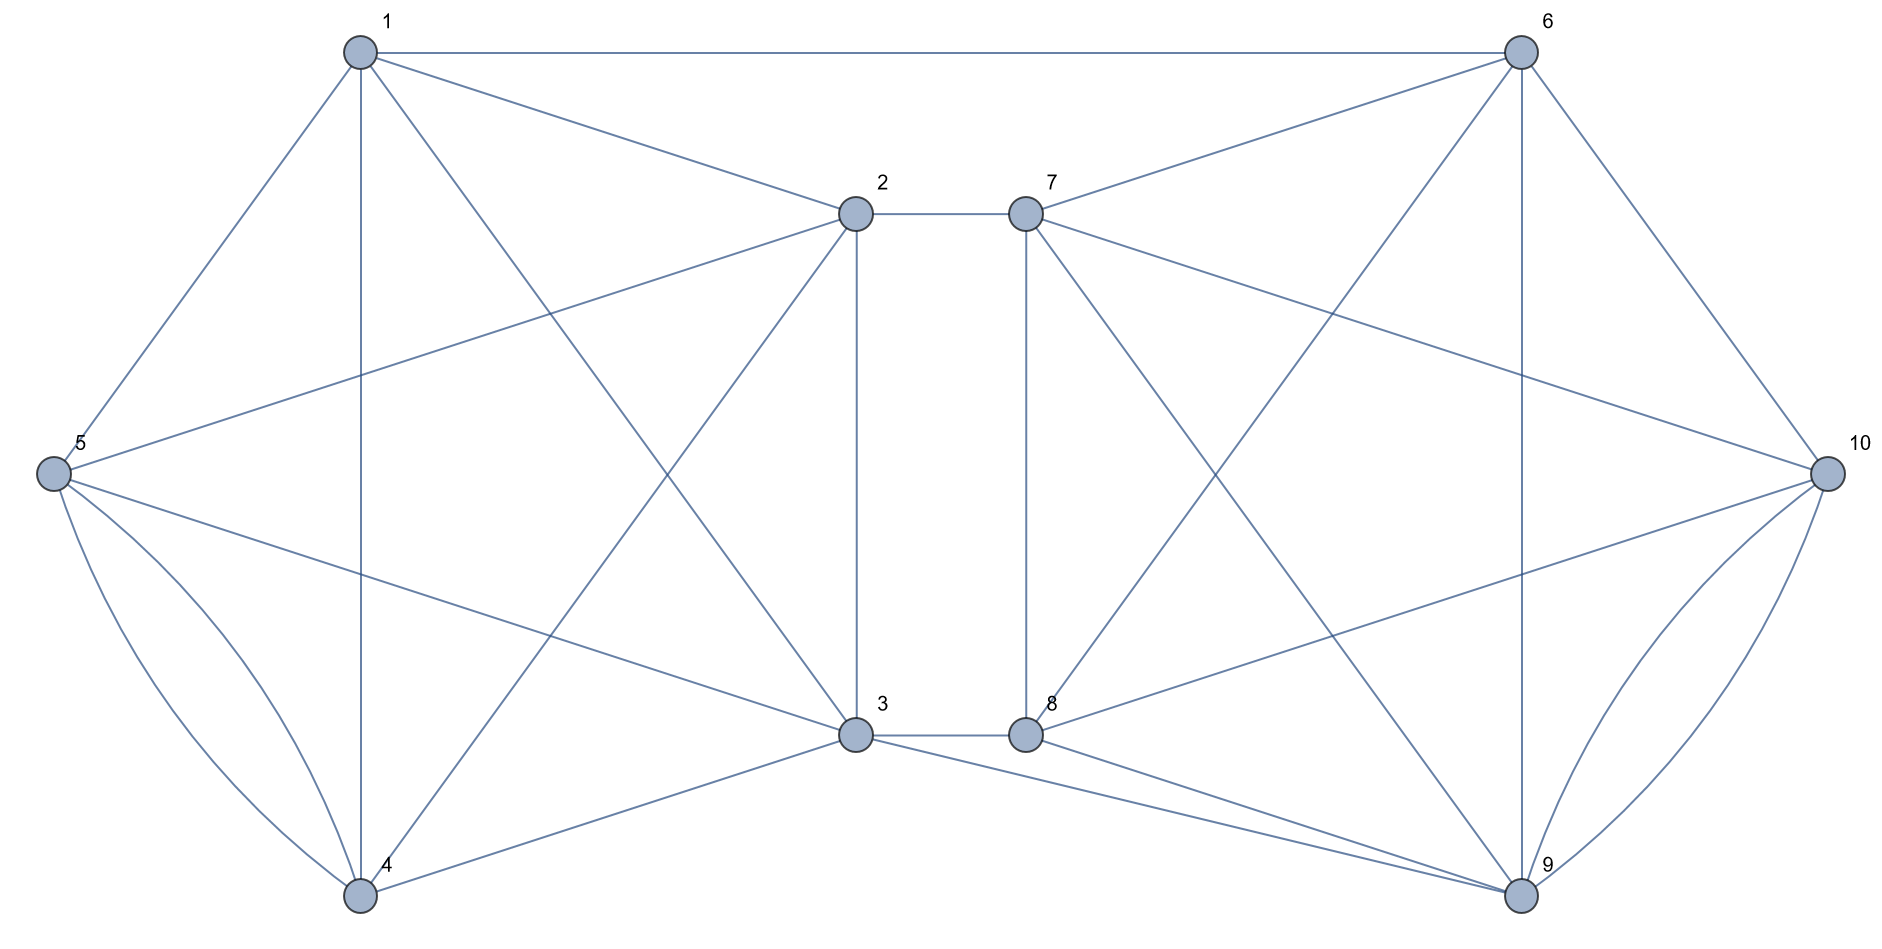
\includegraphics[scale=0.3]{345graph.png}
    \end{center}\vspace{-0.8cm}
\end{proof}

\paragraph{9.3.5}立方图有$\kappa=\kappa'$.
\begin{proof}
    立方图即$d(v)=3(\forall v\in V), \delta=3$,故$\kappa=0,1,2,3$.$\kappa=0$时图不连通,故$\kappa'=0$.$\kappa=1$即图可分,其有割点连接至少两个区块,由$d(v)=3$知与至少一个区块仅以一条边连接,删去此边可使图不连通,从而$\kappa'=1$.$\kappa=3$时由$3=\kappa\leq\kappa'\leq\delta=3$知$\kappa'=3$.
    
    $\kappa=2$时,考虑图的极小点割$S=\cbr{s_1,s_2}$,由极小点割中的点与所有连通分支相邻(见9.1.8的证明),$2\leq c(G-S)\leq d(s_1)=3, c(G-S)=2,3$.记$G-S=\sum_{i=1}^{c}H_i, H_i$为连通分支,则$\forall H_i\forall s_j\in S\exists e_{ij}\in E, e_{ij}\in E(H_i,s_j)$.下对$c(G-S)$分别讨论.
    \begin{itemize}
        \item $c(G-S)=3$时由$d(s_j)=3$知$E(H_i,s_j)=\cbr{e_{ij}}$.故从$G$中删去$e_{i1},e_{i2}$后$\partial(H_i)=E(H_i,G-H_i)=E(H_i,S)=\varnothing$,即$G-\cbr{e_{i1},e_{i2}}$中$H_i$是连通分支.故$\kappa'=2$.
        \item $c(G-S)=2$时,由$d(s_j)=e(s_j,H_1)+e(s_j,H_2)+e(s_j,s_{j'})=3$及抽屉原理知,$\forall s_j\in S\exists H_{i_j}, e(s_j,H_{i_j})=1$.
        
        若存在$i_1=i_2=i, E(H_i,S)=\cbr{e_{i1},e_{i2}}$,则$G-\cbr{e_{i1},e_{i2}}$中$\partial(H_i)=\varnothing$,即$G-\cbr{e_{i1},e_{i2}}$不连通.
        
        若不存在,即$i_1\neq i_2$,则$e(s_1,H_{i_2})=e(s_2,H_{i_1})=2, e(s_1,s_2)=0$,从而$H_{i_1}+s_1+e_{i_11}$与$H_{i_2}+s_2+e_{i_22}$为$G-\cbr{e_{i_11},e_{i_22}}$的分支.故$\kappa'=2$.
    \end{itemize}\vspace{-0.8cm}
\end{proof}

\section{第十章\; 平面图}
\paragraph{10.2.4}$G$是平面图,则$G^{**}\cong G\iff G$连通.
\begin{proof}
    $\implies:$平面图的对偶总是连通的,因为$V(G^*)=F(G)$中的面可以经过有限步长与唯一的外面(outer face)相邻,故$G^*$中的点总与外面对应的点间有路.而连通图的对偶连通,故$G\cong G^{**}$连通.

    $\impliedby:$注意到$G^{**}$的点对应于$G^*$的面,而后者边界上的每条边都要在平面上仅经过一条$G$中的边,且$G$中的边也要经过一条$G^*$的边,从而由Jordan曲线定理知$G^*$的面边界内有且仅有一个$G$的点,因此有$V(G^{**})$与$V(G)$之间的对应.而$G^{**}$中点通过边$e^{**}$相邻等价于$G^*$中面通过边$e^{*}$相邻,等价于$G$中的点通过边$e$相邻,即边集之间有对应关系且保持相邻关系.综上所述$G^{**}\cong G$.
\end{proof}

\paragraph{10.3.2}(1)连通平面图$G$的最短圈长(girth)$k\geq 3$,证明$m\leq \frac{k(n-2)}{k-2}$.(2)证明Petersen图不是平面图.
\begin{proof}
    注意到圈$\partial(f)$长$d(f)\geq k$,故
    $$2m=\sum_{f\in F}d(f)\geq kf=k(2+m-n), (n-2)m\geq (k-2)n, m\leq \frac{k(n-2)}{k-2}$$
    而Petersen图有$n=10,m=15,k=5$,即$\rhs=40/3<15=m$,从而不是平面图.
\end{proof}

\section{第十六章\; 匹配}
\paragraph{16.1.5}(1)$M,M'$是图$G$的最大匹配,描述子图$H=G[M\triangle M']$的结构.\\
(2)$M,M'$是图$G$的完美匹配,描述子图$H=G[M\triangle M']$的结构.\\
(3)由(2)证明树有至多一个完美匹配.
\begin{proof}
    (1)由于$H$中点的度数仅可能为1或2,故$H$中连通分支仅可能有路和圈.而对于点$v\in V(H), d(v)=2$即其连接$M$与$M'$中各一条边,故所有路和圈都是交错的,从而均为偶长度.

    (2)完美匹配也是最大匹配,故$H$中仅可能有$M$-交错路或圈.若有交错路,则其首端点不被$M$或$M'$覆盖,与完美匹配矛盾,故不存在交错路,仅存在交错圈.

    (3)若取$G$是树,$M,M'$是其两个完美匹配,则$H$中不可能含圈,即$H=\varnothing$,从而$M=M'$.
\end{proof}

\paragraph{16.1.7}$M$是图$G$的完美匹配,$S\subset V$,证明$\abs{M\cap\partial(S)}\equiv \abs{S}\bmod 2$.\\
(2)若$M$是Petersen图的完美匹配, $C$是图中一个5-圈的边集,则$\abs{M\cap C}$是偶图.
\begin{proof}
    (1)$s\in S$都被$M$覆盖,故$s$是$M\cap\partial(S)$中边的端点或$M\cap E(S)$中边的端点,且不可能同时是两者中边的端点.而$e\in M\cap\partial(S)$在$S$中的端点仅有1个,$e\in M\cap E(S)$在$S$中的端点有2个,故
    $$\begin{aligned}
        \abs{S}&=\#\cbr{v\in S|v被M\cap\partial(S)覆盖}+\#\cbr{v\in S|v被M\cap E(S)覆盖}=\abs{M\cap\partial(S)}+2\abs{M\cap E(S)}\\
        &\equiv \abs{M\cap\partial(S)}\bmod 2
    \end{aligned}$$

    (2)由上知$\abs{M\cap \partial(C)}+2\abs{M\cap C}=v(C)=5,\abs{M\cap C}=0,1,2$,故即证$\abs{M\cap C}\neq 1, \abs{M\cap \partial(C)}\neq 3$.记$C=u_1u_2u_3u_4u_5u_1$,由于Petersen图是3-正则图,故$C$中每个点都与$C$外一点相邻,记$u_i$在$C$外的邻点为$v_i$.若$\abs{M\cap C}=1$,不失一般性的,记$M\cap C$中唯一边为$e=u_1u_2$,而$u_3,u_4,u_5$均被$M\cap \partial(C)$覆盖,故$u_1u_2,u_3v_3,u_4v_4,u_5v_5\in M$,而$v_1,v_2$不相邻(否则Petersen图有4-圈$u_1u_2v_2v_1u_1$),这与$M$完美矛盾,故得证.
\end{proof}

\paragraph{16.1.15}称$v\in V$为必要点(essential vertex),若其被$G$的所有最大匹配覆盖,即$\alpha'(G-v)=\alpha'(G)-1$.\\
(1)给出无穷个不含必要点的连通图.(2)证明每个非空二部图都有必要点.
\begin{proof}
    (1)奇圈图的最大匹配总不匹配其中一点,故对其上任意点都可构造对应的最大匹配不含该点,即奇圈图不含必要点.

    (2)记二部图为$G[X,Y]$,取最大匹配$M$,存在点$x\in X$不被其覆盖(否则为完美匹配,命题自然成立),则$N(x)\subset Y$被$M$覆盖,否则$\exists y\in N(x), xy$为$M$-增广路,矛盾.再取最大匹配$M'$,若其不覆盖$x$则同理$M'$覆盖$N(x)$.若$M'$覆盖$x$,下证$N(x)$同样被$M'$覆盖,从而$N(x)$总为必要点.

    若存在$y\in N(x)$不被$M'$覆盖,而其被$M$覆盖,故$\exists x_1\in X-\cbr{x}, yx_1\in M$,故$yx_1\in M\triangle M'$.由$M\triangle M'$中路长度为偶数知,有路$yx_1y_1\subset M\triangle M'$,即$x_1y_1\in M'$.若$y_1$不被$M$覆盖,则$xyx_1y_1$是$M$-增广路,矛盾,故$\exists x_2\in X-\cbr{x,x_1}, y_1x_2\in M$.以此类推,$M\triangle M'$有路$xyx_1y_1x_2y_2\cdots$,但$M\triangle M'$有限,从而矛盾.
\end{proof}

\paragraph{16.2.7}二部图$G=G[X,Y]$有最大匹配$M^*$,$U\subset X$不被$M^*$覆盖.记从$U$中顶点通过$M^*$-交错路可达的点构成点集$Z$,$R=X\cap Z, B=Y\cap Z$.证明(1)$K^*=(X-R)\cup B$是覆盖.(2)$\abs{K^*}=\abs{M^*}$.
\begin{proof}
    (1)若存在$e=xy\in E, x\in X-K^*=R, y\in Y-K^*=Y-B$,则存在从$u\in U$到$x$的$M^*$-交错路$P$,讨论奇偶性知$\exists y'\in Y, y'x\in M$.而$y\notin B$即不存在$U$到$y$的$M^*$-交错路,$P+e$不是$M^*$-交错路,故$e\in M$,矛盾于匹配定义.从而$V-K^*$的点之间不存在边.

    (2)已知$\abs{K^*}\geq\abs{M^*}$,即证$\abs{K^*}\leq\abs{M^*}$.而$\abs{K^*}=\abs{X}-\abs{R}+\abs{B}$,由于$R-U$与$B$中点通过交错路一一对应,故$\abs{R-U}=\abs{B}, \abs{R}-\abs{B}=\abs{U}, \abs{K^*}=\abs{X}-\abs{U}$.另一方面,$X$中至多有$\abs{X-U}$个元素被$M^*$覆盖,即$\abs{M^*}\geq \abs{X-U}=\abs{K^*}$,从而得证.
\end{proof}

\paragraph{16.2.11}无孤立点的图的一个边覆盖是与所有点关联的边构成的边集,图$G$中最小边覆盖中边的个数记作$\beta'(G)$.证明对无孤立点图都有$\alpha'+\beta'=n$.
\begin{proof}
    首先证明任意最小边覆盖$F$中含有最大匹配.考虑生成子图$G[F]$的最大匹配$M$,其也为$G$的匹配.注意到$\forall e\in F-M$的端点不能都被$M$匹配,否则$e$的端点均在$F$中,从而$F-e$仍为边覆盖,与$F$最小矛盾;也不能都不被$M$覆盖,否则其为$M$-增广路,与$M$最大矛盾.因此$e\in F-M$的端点能且仅能被$M$覆盖一个.
    
    下证$M$为$G$的最大匹配.若否,则$G$中有长$2k+1$的$M$-增广路$P$.由于$P$的首尾端点$u,v$均被$F$覆盖而不被$M$覆盖,故有边$uu_1,vv_1\in F-M$,由上知$u_1,v_1$被$M$覆盖.且$uu_1,vv_1$均不在$P$中,否则$P$成为$F$中的$M$-增广路,矛盾于$M$在$F$中最大.综上所述,取$F'=(F-M\cap P-\cbr{e_1,e_2})\cup (P-M)$,其为$G$的边覆盖,因为$V(P)$被$P-M$覆盖,其余点被$F-M\cap P$覆盖.而$\abs{F'}<\abs{F}$,矛盾于最小性,从而$M$是$G$的最大匹配.

    最后证明问题:取最小边覆盖$F$中$G$的最大匹配$M$,$U$是未被$M$覆盖的点集,注意到$U$中的点与$F-M$中的边一一对应,故有$\beta'=\abs{F}=\abs{M}+\abs{F-M}=\alpha'+\abs{U}$.再对被$M$覆盖的点集计数,由于,有$n-\abs{U}=2\abs{M}=2\alpha'$.综上可知$\alpha'+\beta'=2\alpha'+\abs{U}=n$,得证.
\end{proof}

\section{第十八章\; Hamilton圈}
\paragraph{18.1.3}证明Meredith图不是Hamilton图. %Fig 17.6
\begin{proof}
    注意到Meredith图是10个$K_{3,4}$以Peterson图的方式连接起来,而Peterson图无Hamilton回路,故若Meredith图有Hamilton回路$P$,则其中一个$K_{3,4}$图被$P$经过至少两次.而每个$K_{3,4}$图与其他部分仅以4个点连接,且4个点都在一个partite set $X$中,而$P$仅可从连接点出入,每次出入仅能经过partite set $Y$中一个点,故$Y$中三个点不能全被遍历.从而Meredith图没有Hamilton回路.
\end{proof}

\paragraph{18.3.5}$G$是简单图,证明(1)若$G$连通且$\delta\leq \frac{n-1}{2}$,则$G$中有长$2\delta$的路.(2)若$\delta\geq \frac{n-1}{2}$则$G$是可追踪(traceable)图.
\begin{proof}
    (1)证明有误待补.
    % (1)取$G$中最长路径$P=v_1\cdots v_\ell$,若$\ell<2\delta\leq n-1$,由于路外的点$u\in V-P$不与$v_1,v_\ell$连接,否则与$P$最长矛盾,因此$u$与$P-\cbr{v_1,v_\ell}$中$\geq\delta-(n-\ell-1)$个点连接.再取$S^-=\cbr{v_i|v_{i+1}与u连接}\subset \cbr{v_1,\cdots,v_{\ell-2}},\abs{S^-}\geq \delta+\ell+1-n$.而$v_\ell$仅与$P$中点连接(否则矛盾于$P$最长),故$v_{\ell}$与$\cbr{v_1,\cdots,v_{\ell-2}}$中$\geq \delta-1$个点连接.故
    % $$\begin{aligned}
    %     \abs{S^-\cap N(v_{\ell})\cap \cbr{v_1,\cdots,v_{\ell-2}}}&=\abs{S^-}+\abs{N(v_{\ell})\cap \cbr{v_1,\cdots,v_{\ell-2}}}-\abs{S^-\cup (N(v_{\ell})\cap \cbr{v_1,\cdots,v_{\ell-2}})}\\
    %     &\geq\abs{S^-}+\abs{N(v_{\ell})\cap \cbr{v_1,\cdots,v_{\ell-2}}}-\abs{\cbr{v_1,\cdots,v_{\ell-2}}}\\
    %     &\geq (\delta+\ell+1-n)+(\delta-1)-(\ell-2)=2\delta-n+2\geq 1
    % \end{aligned}$$
    % 从而可取到$v_i\in V(P)$与$v_{\ell}$连接,且$v_{i+1}$与$u$连接.从而可取路$P'=v_1\cdots v_iv_{\ell}v_{\ell-1}\cdots v_{i+1}u$,其比$P$更长,矛盾.故$P$至少长$2\delta$.

    (2)在$G$外另取一点$v$并将其与$G$中所有点连边,得到的图$G+v$满足$\delta(G+v)\geq n/2$,从而由Dirac定理知其有Hamilton圈,从中删去$v$后$G$中有Hamilton路,即得证.
\end{proof}

\paragraph{18.3.6}图$G$有$\alpha\leq\kappa+1$(其中$\alpha$和$\kappa$分别是图的稳定性数与连通度),证明$G$是可追踪图.
\begin{proof}
    在$G$外另取一点$v$并将其与$G$中所有点连边,得到的图$G+v$有$\alpha(G+v)=\alpha(G)\leq \kappa(G)+1=\kappa(G+v)$,从而由Chvátal-Erdős定理知$G+v$有Hamilton圈,从中删去$v$后$G$中有Hamilton路,即得证.
\end{proof}

\paragraph{18.3.9}简单二部图$G=G[X,Y]$满足$\abs{X}=\abs{Y}\geq 2$,其度数序列为$(d_1,d_2,\cdots,d_n), d_1\leq d_2\leq\cdots\leq d_n$.若不存在整数$k\leq n/4$使得$d_k\leq k, d_{n/2}\leq n/2-k$,证明$G$是Hamilton图.\footnote{HINT: Form a new graph H from G by adding edges between all pairs of vertices of X. Show that H is hamiltonian if and only if G is hamiltonian.}
\begin{proof}
    
\end{proof}

\newpage
\section{期末考试}
\paragraph{1} 证明Ramsey数$R(3,3)=6$.
\paragraph{2} Exercise 18.3.5a
\paragraph{3} Exercise 1.3.15a
\paragraph{4} Exercise 2.5.5
\paragraph{5} Exercise 4.3.5a
\paragraph{6} Exercise 5.2.11
\paragraph{7} Exercise 9.1.8
\paragraph{8} Exercise 9.3.5
\paragraph{9} Exercise 16.2.11
\paragraph{10} 若非完备图$G$中点$u,v$有$d(u,v)=2$都有$d(u)+d(v)\geq n$,证明$G$是Hamilton图.
\end{document}